%%%%%%%%%%%%%%%%%%%%%%%%%%%%%%%%%%%%%%%%%
% University/School Laboratory Report
% LaTeX Template
% Version 3.0 (4/2/13)
%
% This template has been downloaded from:
% http://www.LaTeXTemplates.com
%
% Original author:
% Linux and Unix Users Group at Virginia Tech Wiki 
% (https://vtluug.org/wiki/Example_LaTeX_chem_lab_report)
%
% License:
% CC BY-NC-SA 3.0 (http://creativecommons.org/licenses/by-nc-sa/3.0/)
%
%%%%%%%%%%%%%%%%%%%%%%%%%%%%%%%%%%%%%%%%%

%----------------------------------------------------------------------------------------
%	PACKAGES AND DOCUMENT CONFIGURATIONS
%----------------------------------------------------------------------------------------

\documentclass{article}

\usepackage[version=3]{mhchem} % Package for chemical equation typesetting
\usepackage{siunitx} % Provides the \SI{}{} command for typesetting SI units

\usepackage{graphicx} % Required for the inclusion of images
\usepackage{caption}
\usepackage{subcaption}
\usepackage{cancel}

\usepackage{float}

\usepackage[T1]{fontenc} % allow small bold caps

\setlength\parindent{0pt} % Removes all indentation from paragraphs

\renewcommand{\labelenumi}{\alph{enumi}.} % Make numbering in the enumerate environment by letter rather than number (e.g. section 6)

%\usepackage{times} % Uncomment to use the Times New Roman font

%----------------------------------------------------------------------------------------
%	DOCUMENT INFORMATION
%----------------------------------------------------------------------------------------

\title{Mobile Diagnostic Tools for Pulmonary Disease\\ UAP Proposal} % Title

\author{Ryan Lacey}

\date{}

\begin{document}

\maketitle % Insert the title, author and date

\begin{center}
\begin{tabular}{l r}
Advisor: & Dr. Rich Fletcher \\
Proposed: & March 7, 2014 \\
\end{tabular}
\end{center}

\section{Objective}

The purpose of this project is to develop a mobile application for use in clinics with limited resources in developing regions of India. The application will serve as a diagnostic tool for clinicians trained in Ayuverdic medicine to diagnose patients suffering from a pulmonary disease. With an Android mobile device and a low cost digital stethoscope these clinicians will be able to collect patient lung sounds, run diagnostic machine learning algorithms on the lung sound data, and receive classification feedback with the objective of early detection of the onset of pulmonary disease.\\

\section{Motivation}

Pulmonary diseases (asthma, pneumonia, lung cancer, tuberculosis, etc.) are an increasing concern in the realm of global health challenges. Chronic obstructive pulmonary disease (COPD) alone is currently the third leading cause of death in the world and second leading cause of death in India. Pneumonia, which also affects the lungs, remains the leading cause of death in Indian children under the age of five. Especially at risk are low income populations due to consequences of living environment, lack of access to health care, and the high cost of screening tools for detection of these diseases.\\

There is a great need to provide health workers in India a simple tool that can be used to screen for respiratory disease in the primary care setting and identify individuals that require clinical examination and intervention. Since a majority of the clinicians practice Ayuverdic medicine they have little training for diagnosing respiratory problems. As a result many patients go undiagnosed or are misdiagnosed with having a cardiac disease. The disease burden can be significantly reduced if there were better tools that could perform early detection of respiratory disease and enable clinical intervention before the disease became more critical or developed further into chronic disease.\\

\section{Goals}
\begin{enumerate}
\item[] \texttt{Phase I}\\ Utilize machine learning algorithms to classify common disease states.
\item[] \texttt{Phase II} \\ Integrate digital monitors into application.
\item[] \texttt{Phase III} \\ Develop graphical user interface for Android mobile devices.
\end{enumerate}

Phase I of the project is to develop the tools necessary for patient data to be analyzed. The most fundamental function of the application is for machine learning algorithms to give a binary classification of the data, ie. either the patient has the disease or the patient does not suffer from the disease. Since these classifiers only state "yes or no" instead of "which", each disease will require its own classifier. The most common technique for this type of classification is a simple linear classifier called a support vector machine (SVM). The SVM will train on pre-classified data of Indian patients with the target diseases and aims to minimize potential misclassification of future patients based off of the sample data. Since there are no known machine learning libraries for Android devices a large portion of the work for this project will be in the implementation, training, and testing of these algorithms. \\

Phase II involves converting audio signals from the digital stethoscope into data for the machine learning algorithms. The stethoscope records data at four locations on the patient's body: the front, side, back, and throat. Lung sound data, as seen in \texttt{Figure 1}, will be ran through a pattern recognition algorithm that identifies crackle, wheeze, and plural rub. The output is a two-dimensional matrix incorporating time and sound information from which features can be extracted for the learning algorithm.\\

\begin{figure}[H]
\minipage{\textwidth}
	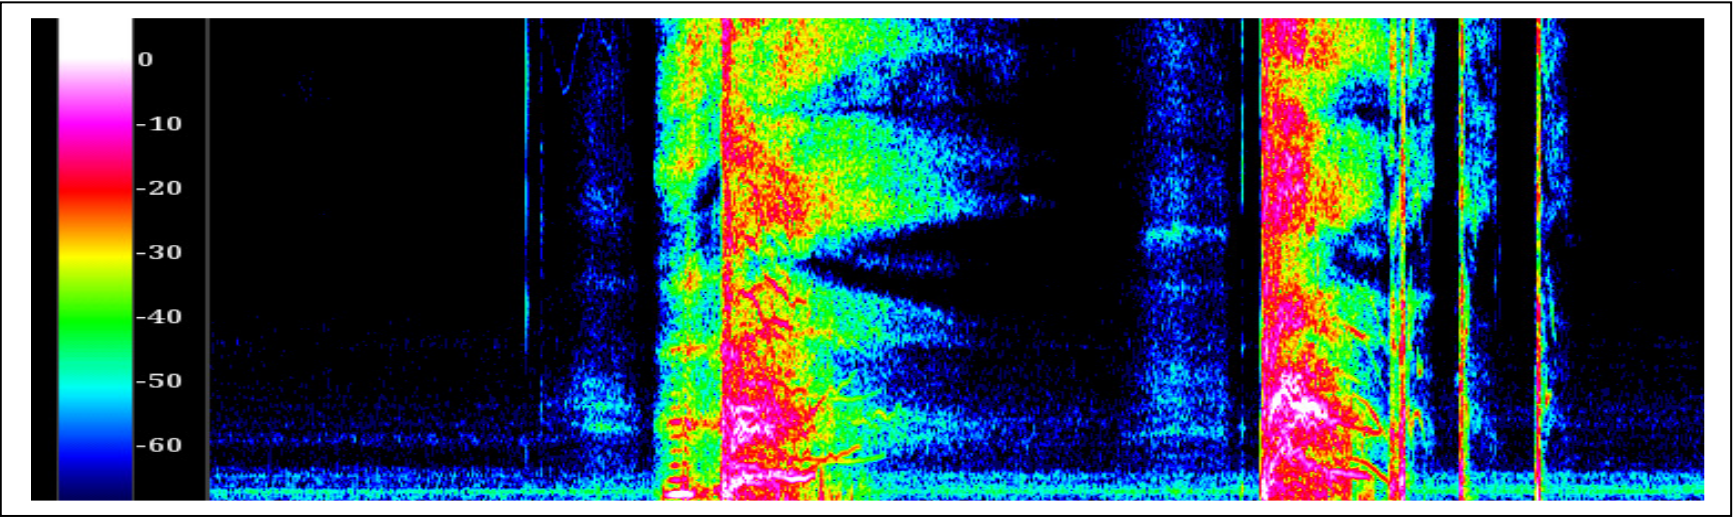
\includegraphics[width=\linewidth]{images/LungSounds.png}
	\caption{Raw data from lung sounds showing time-frequency plot.}
\endminipage\hfill
\end{figure}

Phase III is the most open ended portion of the project. Development of an intuitive user interface is always an iterative process and is likely to continue as feedback is gathered from the test users and eventually the target clinician group. The first task is to create a skeleton interface that will allow for basic functionality to be realized once the data connection between the monitor and the mobile device is completed. This includes the main view of the application, any menus necessary for operation, and the first steps in graphical displays of patient data. The GUI will be developed in Java using the Android SDK for use on phones and tablets. The ultimate goal is for the interface to be intuitive and language independent so that individuals with limited technological experience will be able to utilize the application. \\

\end{document}